% -------------------------------------------------------------------------
% Section: Modeling the Variability Mechanisms
% ------------------------------------------------------------------------
\section{SVCM Approach}
\label{sec:svmc}

To solve the problems mentioned in the previous section, we introduce now our
approach for modeling variabilities in use case scenarios, which was named
\emph{Modeling Scenario Variability as Crosscutting Mechanisms} (MSVCM). It
improves the separation of concerns between variability management and scenario
specifications, dealing with scenario variability as a composition of different
artifacts: SPL use case model, feature model, product configuration,
and configuration knowledge.

Motivated by the Masuhara and Kiczales (MK) work~\cite{Masuhara:2003aa}, our
approach for \textbf{scenario variability management} relies on a weaving
process that takes as input the aforementioned artifacts, which crosscut
each other with respect to the resulting product specific use case model
(Figure~\ref{fig:weave-process}). Combining these input artifacts, it is possible
to represent the sources of variability that we are interested in:
\emph{variability in function}, \emph{variability in data}, and \emph{variability in
control flow}~\cite{Bachmann:2001aa}.

\begin{figure}[htb]
 \begin{center}
  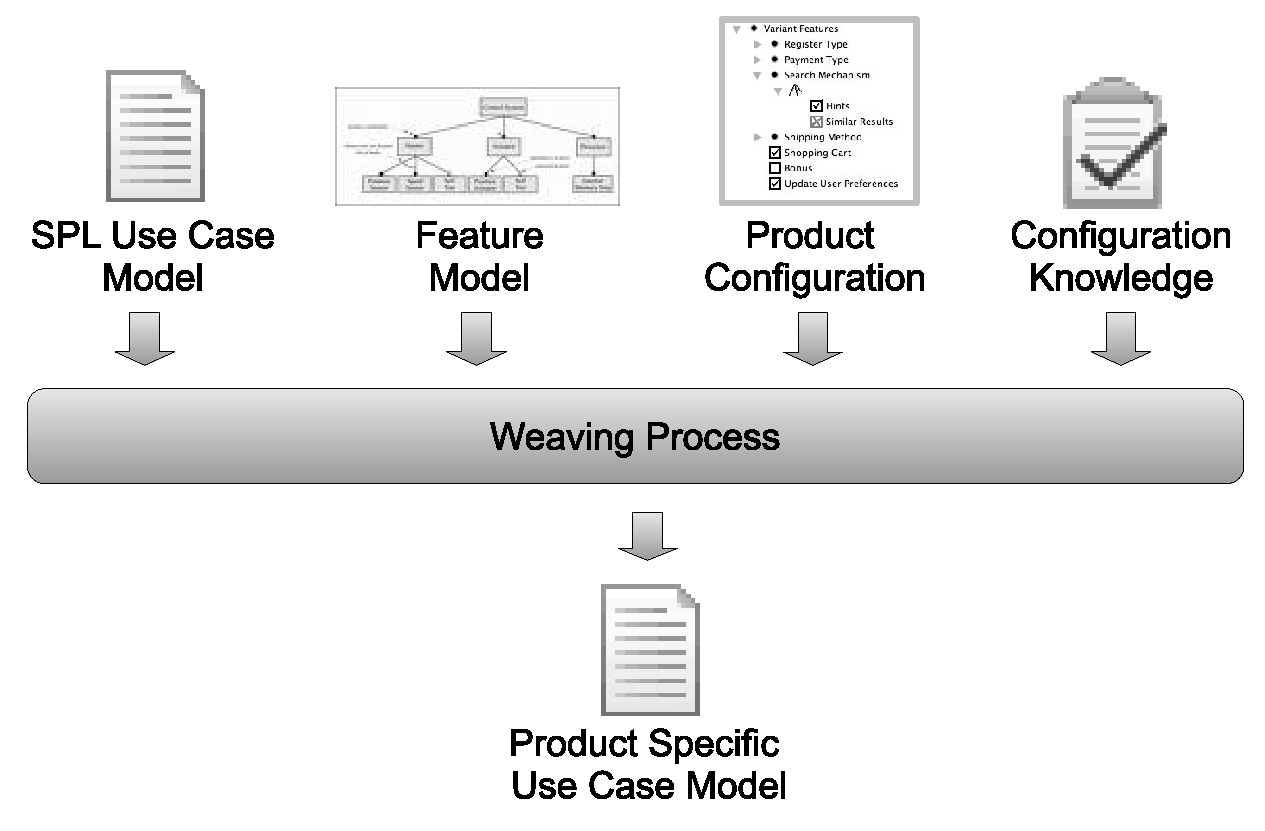
\includegraphics[scale=0.30]{img/weave-process2.eps}
  \caption{Overview of our weaving process.}
  \label{fig:weave-process}
  \end{center}
\end{figure}

\newpage

The semantics of the weaving process (and the
meta-model of the input and output languages) are described using the Haskell
programming language. This led to concise descriptions and kept our model close
to the MK work, where their weaving processes are specified using Scheme---
another functional programming language. The choice for Haskell was motivated by
several factors, such as improved readability and our background in the language.
The resulting source code is available at a web site~\cite{SPG:site}. In what follows, we detail our approach showing
how it can be used to specify the motivating example. Several artifacts of each
input model are shown; mentioning the contribution of these models to the whole
weaving process.

% {\color{red} With
% respect to the supporting tools, instances of the input models are specified
% using \emph{widespread} tools, and then imported to our variability
% management environment. In this section, we also explain which are these tools and present
% the layered architecture of the Haskell libraries used in our environment.} After
% that, in Section~\ref{sec:modeling-framework} we describe the semantics of our
% approach using a slight customization of the MK framework.



\subsection{Feature model}

Feature models have an important contribution to our weaving process, since they
are used for checking if a product configuration is a valid member of the product
line. We have implemented specific functions in Haskell to deal with
this kind of validation. Basically, these functions verify if all constraints defined in
a feature model are satisfied by a product configuration. 

The code fragment below presents the signature of the \emph{topmost} function
for checking instances of a feature model. It states that
\texttt{checkConfiguration} takes as input a feature model (\emph{FM}) and a
product configuration (\emph{PC}), returning all constraints that a
\emph{PC} does not satisfy. If a \emph{PC} complies with the \emph{constraints}, the
function returns an empty list.

\begin{code}
checkConfiguration :: FM -> PC -> ErrorList
\end{code}

Going into details, the \texttt{checkConfiguration} function traverses two
\emph{rose trees}~\cite{Hinze:2007aa}, representing both feature model and
product configuration, at the same time that it calls specific functions for
checking the rules applied for each type of feature relationship
(mandatory, exclusive or, inclusive or) and constraints. 


Although we are not proposing a new notation for feature modeling, we
had to create specific data types for feature models in Haskell.  The same was
true for the other input models of our weaving process. For instance, the code
bellow shows the feature model data type. It basically consists of a root feature
and a list of global constraints. Due to lack of space, in this paper we do not
present all input model data types.

\begin{code}
data FeatureModel = FeatureModel {
	root :: Feature,
	constraints :: [Constraint]
} 
data Feature = Feature  { 
  id :: Id, 
  name :: Name, 
  featureType :: FeatureType,-- (optional, mandatory)
  featureGroup :: Group,-- (none, ior, xor)
  children :: [Feature]
} 
 \end{code}
 
Additional functions were defined for importing feature models, generated by the
\emph{Feature Modeling Plugin} (FMP)~\cite{Czarnecki:2004aa}, to our
environment. In the remainder of this section, we consider the \emph{eShop}
feature model introduced in the motivating example (Figure~\ref{fig:eshop-fm}). 

%For
%instance, {\color{blue}Based on the feature model of Figure~\ref{fig:eshop-fm},
%the \emph{Shopping Cart}, \emph{Bonus} and \emph{Update User Preferences}
%features are optional; on the other hand, the \emph{Shipping Method} feature is
%mandatory and all products have to be configured with at least one of its child.
%Additionally, the restriction $Shopping\ Cart\ \Leftrightarrow\ Bonus$ states
%that all products configured with the shopping cart feature must also be
%configured with the bonus feature. More details about feature modeling can be
%found elsewhere~\cite{Gheyi:2006aa,Czarnecki:2000aa}.}

\subsection{SPL use case model}\label{sub:spl-uc}

This artifact defines scenarios that describe the expected behavior of the SPL's
members. Scenarios might be optional, have parameters, and change (advice) the
behavior of other scenarios. A use case model is composed by \emph{use cases} and
\emph{aspectual use cases}. A use case has a name, a description and a list of
scenarios, which are composed by a sequence of steps (pairs of \emph{User action x
System response}). An aspectual use case has a name and a list of advices, which
can be used to extend the behavior of existing scenarios.

Differently from PLUSS, which directly relates alternative and
optional steps to features, in our approach \emph{feature} and \emph{use case
models} are syntactically independent from each other. There is no direct
association joining these models and all relationships between them are kept by
the configuration knowledge (Section~\ref{sub:configuration-knowledge}).
 Actually, the weaving process, whose semantics are presented in
 Section~\ref{sec:modeling-framework}, is responsible for binding the variation
 points defined in the SPL use case model. In order to do that, other assets
 (such as product configurations and configuration knowledge) have to be
 considered.

Regarding tool support, instances of the use case model can
be written in any text editor that is able to export documents using a specific
XML format\footnote{Templates are available for Microsoft Word.}. Additional functions were
developed for parsing these documents to the abstract data type of our use case
model.

In this running example, we consider the following scenarios and advices:

{\bf Proceed to Purchase:} this mandatory scenario
(Figure~\ref{fig:proceed-to-checkout}) specifies the common behavior that is
required for confirming a purchase. Instances of the product line must be
configured with this scenario. 
Notice that a parameter (\emph{SM}) is referenced in Step P2. 
This parameter allows the reuse of the \emph{Proceed to
Purchase} scenario for different configurations of the \emph{Shipping Method} feature. Parameters 
are also supported in PLUSS and PLUC. However, in these approaches parameters are directly related to features or members of the product line.

The annotation \mbox{\texttt{[CustomerPreferences]}} (Step P3) is
another variation point of \emph{Proceed to Purchase} scenario. This annotation, also assigned to the Step S3 of \emph{Search for Products} (Figure~\ref{fig:search-products-flow}), reveals points in the specification that are related to the customer preferences. Since pointcuts can make references to annotations, the advice \emph{Register User Preferences} (Figure~\ref{fig:register-preferences-flow}) extends the behavior of \emph{Proceed to Purchase} after Step P3. Note that our annotations just reveal variation points, which means that annotated steps are \emph{obliviousness} about which features extend the corresponding behavior. 


\begin{figure}[h]
\begin{scriptsize}
  \texttt{
   \begin{tabular}{l}
   	 {\bf Id: SC01} 	\\
     {\bf Description:} Proceed to purchase\\
   \end{tabular}
  \begin{center}
  \begin{tabular}{||p{0.1in}||p{1.4in}||p{1.4in}||}
   \hline
       Id & User Action  & System Response \\ \hline \hline
       P1 & Fill in the requested information and select the proceed option.  & Request the shipping method and address.\\  \hline
       P2 & Select one of the available shipping methods (\mbox{<SM>}),
       fill in the destination address and proceed. & Calculate the shipping costs. \\  \hline P3 & Confirm the purchase. & Execute the order and send a request to the Delivery System to dispatch the products.
       \mbox{[CustomerPreferences]} \\  \hline
  \end{tabular}
  \end{center}
  }
\end{scriptsize}
\caption{Proceed to purchase scenario.}
\label{fig:proceed-to-checkout}
\end{figure}

{\bf Buy Product:} this advice (Figure~\ref{fig:buy-product-scenario}) enables a
customer to buy specific goods from an on-line shopping store. It is only
available in the product line members that are {\bf not} configured with the
\emph{Shopping Cart} and \emph{Bonus} features. The effect of this advice is to
introduce an optional behavior {\bf before} the join points identified in its
\emph{pointcut} clause. In this case, the Step P1 defined in the \emph{Proceed to
Purchase} scenario. Therefore, the \emph{pointcut} clause can refer either to step ids or
step annotations (as explained before). However, we encourage the definition of
pointcuts based on annotations, since they mitigate the problem
of fragile pointcuts. This problem occurs because changes in the order of
steps might break pointcuts.
 
\begin{figure}[h]
\begin{scriptsize}
  \texttt{
   \begin{tabular}{l}
   	 {\bf Id: ADV01} 	\\
     {\bf Description:} Buy a specific product\\
     {\bf Before:}  P1
   \end{tabular}
  \begin{center}
  \begin{tabular}{||p{0.1in}||p{1.4in}||p{1.4in}||}
   \hline
       Id & User Action  & System Response \\ \hline \hline
       B1 & Select the buy product option.  & Present the selected product. The user can change the quantity of items he wants to buy. Calculate and show the amount to be paid. \\  \hline
       B2 & Select the confirm option. &  Request payment information. \\  \hline
    \end{tabular}
  \end{center}
  }
\end{scriptsize}
\caption{Buy product advice.}
\label{fig:buy-product-scenario}
\end{figure}

{\bf Buy Products with Shopping Cart and Bonus:} this advice
(Figure~\ref{fig:buy-product-changing-flow}) allows purchasing products
that have been previously added to a shopping cart. It extends the
behavior of the \emph{Proceed to Purchase} scenario by introducing the specific
behavior required by the \emph{Shopping Cart} and
\emph{Bonus} features. So, this advice is required by products that
are configured with both \emph{Shopping Cart} and \emph{Bonus} features.

\begin{figure}[h]
\begin{scriptsize}
  \texttt{
   \begin{tabular}{l}
   	 {\bf Id: ADV02} 	\\
     {\bf Description:} Buy products using a shopping-cart\\
     {\bf Before:} P1
   \end{tabular}
  \begin{center}
   \begin{tabular}{||p{0.1in}||p{1.4in}||p{1.4in}||}
   \hline
       Id & User Action & System Response \\ \hline \hline
       C1 & Select the checkout option.  & Present the items in the shopping cart and the amount to be paid. The user can remove items from the shopping cart. \\  \hline
       C2 & Select the confirm option. & Request bonus and payment information. \\  \hline
  \end{tabular}
  \end{center}
  }
\end{scriptsize}
\caption{Buy products with shopping cart advice.}
\label{fig:buy-product-changing-flow}
\end{figure}

{\bf Search for Products:} this mandatory scenario
(Figure~\ref{fig:search-products-flow}) allows a customer to search for products.
In order to save space, we only present Step S3, which performs a search based on
the input criteria. Note that, similarly to the Step P3 shown in
Figure~\ref{fig:proceed-to-checkout}, this step is also assigned to the
\mbox{\texttt{ [CustomerPreferences]}} annotation. Therefore, any advice that
points to this annotation extends, at least, the behavior of \emph{Proceed to Purchase} and
\emph{Search for Product} scenarios.

\begin{figure}[ht]
\begin{scriptsize}
  \texttt{
   \begin{tabular}{l}
   	 {\bf Id: SC02} 						\\
     {\bf Description:} Search for products. \\
   \end{tabular}
  \begin{center}
   \begin{tabular}{||p{0.1in}||p{1.4in}||p{1.4in}||}
   \hline
       Id & User Action &  System Response \\ \hline \hline
       \ldots & \ldots  & \ldots \\  \hline
       S3 & Inform the search criteria. &  Retrieve the products that satisfy the search criteria. Show a list with the resulting products. [CustomerPreferences] \\  \hline
  \end{tabular}
  \end{center}
  }
\end{scriptsize}
\caption{Search for products scenario.}
\label{fig:search-products-flow}
\end{figure}



{\bf Register User Preferences:} this advice
(Figure~\ref{fig:register-preferences-flow}) updates the user preferences based
on the user's history of searches and purchases. Its behavior can be started {\bf
after} any step assigned to the \texttt{[CustomerPreferences]} (see the
\emph{pointcut} clause) annotation and is available in products that are
configured with the \emph{Update User Preferences} feature.

\begin{figure}[h]
\begin{scriptsize}
  \texttt{
   \begin{tabular}{l}
   	 {\bf Id: ADV03} 	\\
     {\bf Description:} Register user preferences.\\
     {\bf After}: [CustomerPreferences] \\
   \end{tabular}
  \begin{center}
   \begin{tabular}{||p{0.1in}||p{1.4in}||p{1.4in}||}
   \hline
       Id & User Action &  System Response \\ \hline \hline
       R1 & - &  Update the preferences based on the search results or purchased items. \\  \hline
  \end{tabular}
  \end{center}
  }
\end{scriptsize}
\caption{Register user preferences.}
\label{fig:register-preferences-flow}
\end{figure}

At this point we are able to present some remarks related to our use
case model. As discussed in Section~\ref{sec:problem}, PLUSS and PLUC represent
all valid configurations of a scenario in a single artifact. Differently, using
our approach, we could separate the common behavior required to confirm a
purchase (the base scenario \emph{Proceed to Purchase}) from its variants,
specified in the \emph{Buy Product} and \emph{Buy Product with Shopping Cart}
advices. This allows our specifications to evolve according to the
\emph{Open-Closed} principle~\cite{Meyer:2000aa}; which means that, in our
approach, introducing new product variants require more extensions than changes
to the base scenarios.

Moreover, in this section we have described several
scenarios as being optional or mandatory, being important to emphasize
that, in our approach, this kind of information is not specified in the use case
model. Actually, it is necessary to consider the relationships between features
and scenarios, represented in the configuration knowledge, in order to be aware
of which scenarios are present in a specific product configuration. Finally,
since different advices can make references to a same join point,  interferences
between advices may occur. Nevertheless, the weaving process evaluates each advice in
a sequence defined by the configuration knowledge. For this reason, interferences
between advices are deterministic and do not require specific constructs in the
use case model to deal with them.

\subsection{Configuration knowledge}\label{sub:configuration-knowledge}

This artifact corresponds to a list of configuration items, which
relates feature expressions to tasks (or transformations) used for automatically generating a
SPL member. Consequently, the configuration knowledge guides the weaving
process. For this running example, the configuration knowledge shown in
Table~\ref{tab:eshop-ck} enforces that

\begin{itemize}
\item Both \emph{Proceed to Purchase} (SC01) and \emph{Search for Products}
(SC02) scenarios are mandatory, since their selection is related to the
(mandatory) root feature of the \emph{eShop} product line;

\item The \emph{Buy Product} advice (ADV01) is used in the composition of
products that do not have been configured with both \emph{Shopping Cart} and \emph{Bonus}
features--- if both features were selected for a product, it would be configured
with the \emph{Buy Product with Cart} advice (ADV02). Remember that there is a
mutual dependency between \emph{Shopping Cart} and \emph{Bonus} features. As a
consequence, no product can be configured with just one of them;

\item The \emph{Register User Preferences} advice (ADV03) is not used in a
product composition unless the \emph{Update User Preferences} feature has been
selected; and

\item References to the ``SM'' parameter are bound to the
selected alternatives of the \emph{Shipping Method} feature.

\end{itemize}

\begin{table}[htb]
\begin{small}
\begin{tabular}{||lp{1.4in}||}
\hline
Feature Expression  						& Tasks					 \\ \hline \hline

\multirow{2}{*}{eShop}						& select scenario {\bf SC01} \\
											& select scenario {\bf SC02} \\	 \hline
{\bf not} (Shopping Cart {\bf and} Bonus) 	& evaluate advice {\bf ADV01} \\ \hline 
(Shopping Cart {\bf and} Bonus) 		& evaluate advice {\bf ADV02} 	\\   \hline
Update User Preferences 				& evaluate advice {\bf ADV03} \\     \hline 
\multirow{2}{*}{Shipping Method}		& bind {\bf SM} to {\bf Shipping} \\  
										& {\bf Method}\\ \hline
								
\end{tabular}
\end{small}
\caption{Example of configuration knowledge}
\label{tab:eshop-ck}
\end{table}

Three different tasks are shown
in Table~\ref{tab:eshop-ck}: \emph{select scenario}, \emph{evaluate advice}, and
\emph{bind parameter}. According to Bachmann et
al.~\cite{Bachmann:2001aa}, the first type of task deals with the source of
variability named as \emph{variation in function}, being responsible for
selecting scenarios; the second one deals with \emph{variation in control flow},
being responsible for composing advices at specific join points; and the last one
deals with \emph{variation in data}, being responsible for binding parameters to
features.

The semantics of these tasks are described as crosscutting mechanisms
in Section~\ref{sec:modeling-framework}. Besides that, the configuration knowledge data type is shown bellow. As explained before, it is a list of configuration items, which relate feature expressions to
\emph{tasks}. Actually, the type \texttt{Task} is a synonymous for the
family of functions that receive a \emph{SPL use case model} ($SPL$) and a \emph{product
specific use case model} ($SPLMember$) as parameters; and then returns a
refinement of the product specific model.
 
 % \begin{small}
 \begin{code}
 type ConfigurationKnowledge = [Configuration]
 data Configuration = Configuration {
  exp :: FeatureExpression,
  tasks :: [Task] 	
 }
 type Task = (SPL -> SPLMember) -> SPLMember
\end{code}

Note that feature expressions have to be written in propositional
logic, because it is necessary to express, for example, that the \emph{Buy Products} advice will be evaluated iff the feature expression {\bf ``not ShoppingCart and Bonus''} is true for a specific product configuration.

Indeed, the \emph{weavingProcess} function, whose source code is presented bellow, behaves like a generator that applies 
the appropriate list of tasks ($ts$) for a given product configuration. This means 
that, first of all, it is necessary to verify  ($eval\ pc\ (exp\ c)$) which expressions ($exp\ c$) 
are valid for a specific product configuration ($pc$). After that, the
$stepRefinement$ function composes the sequence of tasks that must be applied. 

\begin{code}
weavingProcess spl fm pc ck =
   stepRefinement [(t spl) | t <- ts] empty 
   where
    ts = concat [tasks c| c <- ck, eval pc (exp c)] 
    empty = (emptyInstance spl pc)
    stepRefinement l m = ...
 \end{code}
 
As a consequence, supposing the list of tasks
 
$ts=[select(SC01),evaluate(ADV01),evaluate(ADV02)]$,
 
the semantics of this hypothetical product would be given by: $p\ =\  f\ (spl,\ g\ (spl,\ h))$, where:
\begin{eqnarray*}
h  & = & (select\ SC01)\ spl\ emptyInstance \\
g  & = & (evaluate\ ADV01) \\
f   & = & (evaluate\ ADV02) 
\end{eqnarray*}

The previous input models are specified during the domain
engineering phase of SPL development~\cite{Clements:2001aa,Pohl:2005aa}. The next
one, on the other hand, is supposed to be designed whenever a specific product
has to be generated.

\subsection{Product configuration}\label{subsub:pc}

This artifact identifies a specific SPL member, which is characterized by a
configuration of features. One important property is that each product
configuration must comply to a feature model (the selected features must obey
the feature model relationships and constraints).

Our tool environment also uses the FMP~\cite{Czarnecki:2004aa} for representing valid configurations
of specific products. Then, these configurations are parsed to our
environment, instantiating the abstract representation of the \emph{product
configuration} input model. Actually, the abstract representation of a product
configuration is basically a tree representing the selected features. For the
\emph{eShop} example, two possible configurations are presented in
Figure~\ref{fig:product-config-01-02}.

 \begin{figure}[h]
 \begin{center}
  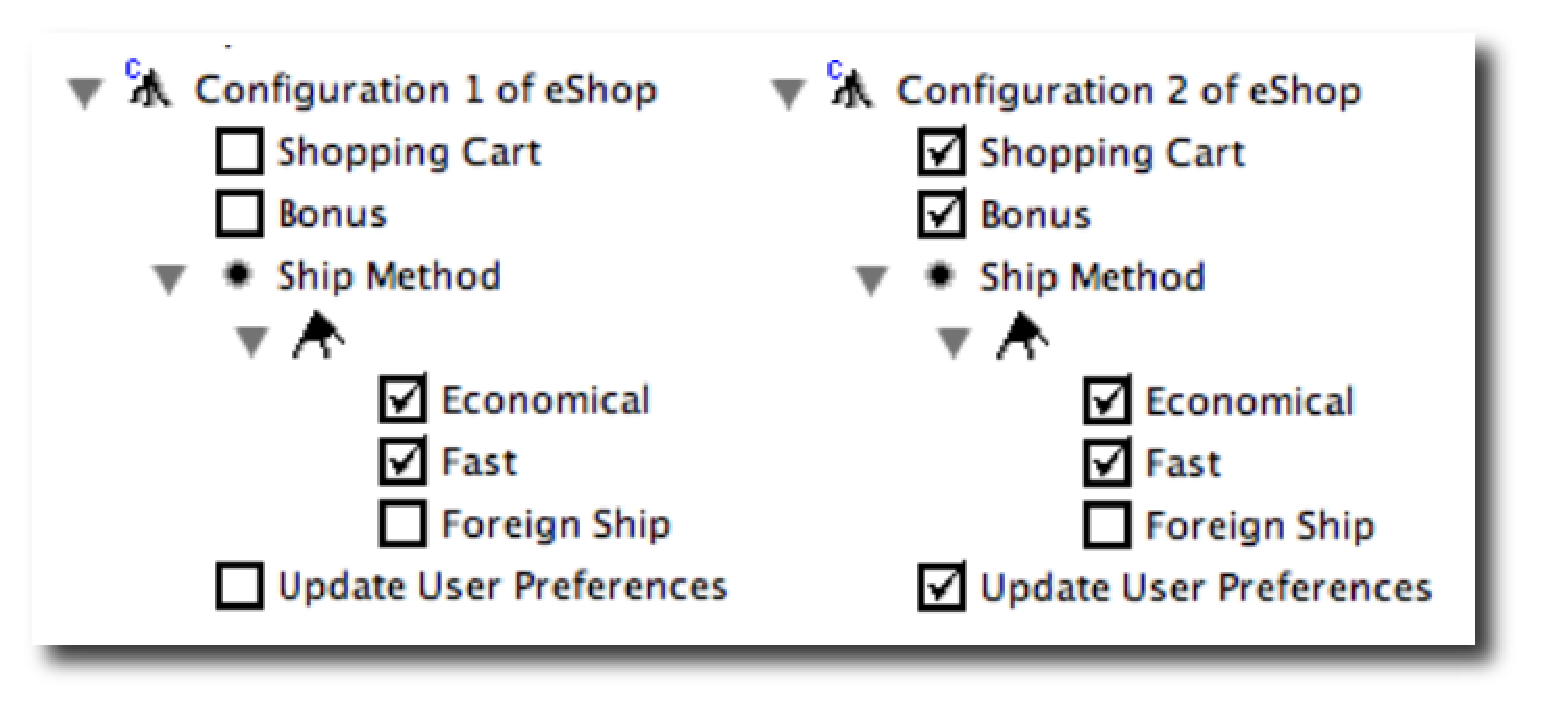
\includegraphics[scale=0.33]{img/pc-04.eps}
   \caption{Examples of product configurations.}
  \label{fig:product-config-01-02}
  \end{center}
\end{figure}

The first configuration (on the left side of the
Figure~\ref{fig:product-config-01-02}) defines a product that does not have support for
\emph{Shopping Cart}, \emph{Bonus} and \emph{Update User Preferences}.
Additionally, it supports only the economical and fast shipping methods. The
second configuration is more complete, being configured with the features
\emph{Shopping Cart}, \emph{Bonus}, and \emph{Update User Preferences}.

As explained in the previous section, the features selected to a specific product
(represented as a product configuration) identify which \emph{tasks} (or
transformations) must be performed in order to generate the corresponding SPL
member. 
Figure~\ref{fig:resulting-scenarios} depicts the resulting scenarios after evaluating the configuration knowledge of
Table~\ref{tab:eshop-ck} and considering the second configuration of
Figure~\ref{fig:product-config-01-02}. According to what was explained in the
previous section, such a configuration requires: 

\begin{enumerate} 
 \item The selection of \emph{Proceed to Purchase} and \emph{Search for Product} scenarios. This selection is directly responsible 
for the resulting scenarios shown in Figure~\ref{fig:resulting-scenarios}. 
  
 \item The evaluation of \emph{Buy Products with Cart} advice. The result of this evaluation is the introduction of the 
first two steps in the resulting specification of the \emph{Proceed to Purchase} scenario. 
 
 \item The evaluation of \emph{Register User Preferences} advice. The result of this evaluation is the introduction of the last steps on both \emph{Search for Products} and \emph{Proceed to
Purchase} scenarios.

 \item The binding of the \emph{SM} parameter to the selected options of the \emph{Shipping Method} feature. This binding is responsible for 
 setting the options \emph{Economical} and \emph{Fast} in the fourth step of the
 resulting \emph{Proceed to Purchase} scenario.

\end{enumerate}

 
\begin{figure}[h]
\begin{scriptsize}
   \texttt{
     \begin{tabular}{l}
   	 {\bf Scenario:} Search for products.\\
      \end{tabular}
   \begin{center}
     \begin{tabular}{||p{0.1in}||p{1.45in}||p{1.4in}||} \hline
      id & User Action  & System Response \\ \hline \hline
       \ldots & \ldots  & \ldots \\  \hline
        3 & Inform the search criteria. &  Retrieve the products that satisfy the search criteria. Show a list with the resulting products. \\   \hline
        4 & - &  Update the preferences based on the search results or purchased items \\\hline 
     \end{tabular}
   \end{center}
   \begin{tabular}{l}
   	 \\
	 {\bf Scenario:} Proceed to purchase.\\
      \end{tabular}
   \begin{center}
     \begin{tabular}{||p{0.1in}||p{1.40in}||p{1.40in}||} \hline
       id & User Action  & System Response \\ \hline \hline
       1 & Select the checkout option.  & Present the items in the shopping
       cart and the amount to be paid. The user can remove items from the
       shopping cart. \\ \hline
       2 & Select the confirm option. & Request bonus and payment information. \\ \hline
       3 & Fill in the requested information and
       select the proceed option.  & Request the shipping method and address.\\ \hline
       4 & Select one of the available shipping methods {\bf (Economical, Fast)}, fill
       in the destination address and proceed. & Calculate the shipping
       costs.\\ \hline
       5 & Confirm the purchase. & Execute the order and send a
       request to the Delivery System to dispatch the products. \\ \hline
 	6 & - &  Update the preferences based on the search results or purchased
 	   items. \\ \hline
    \end{tabular}
   \end{center}
   }
\end{scriptsize}
\caption{Resulting scenarios of the example}
\label{fig:resulting-scenarios}
\end{figure}	

The next section details the semantics of our
weaving process, modeling each source of scenario variability as a crosscutting 
mechanism.

%=====================================================
% TOOL Support
%=====================================================

% \subsection{Tool support}
% 
% {\color{red}As explained before, we are using external tools for specifying 
% features models, use case models, and product configurations. Therefore, only 
% the configuration knowledge is written using the tool support
% {\color{blue}developed for testing the ideas presented in this paper.} 
% 
% Besides allowing the users to specify configuration models, the tool 
% parses the input models from XML documents and starts the weaving process.
% Figure~\ref{fig:graphical-environment} shows the graphical environment that
% integrates these functionalities.
% 
% \begin{figure}[h]
%  \begin{center}
%   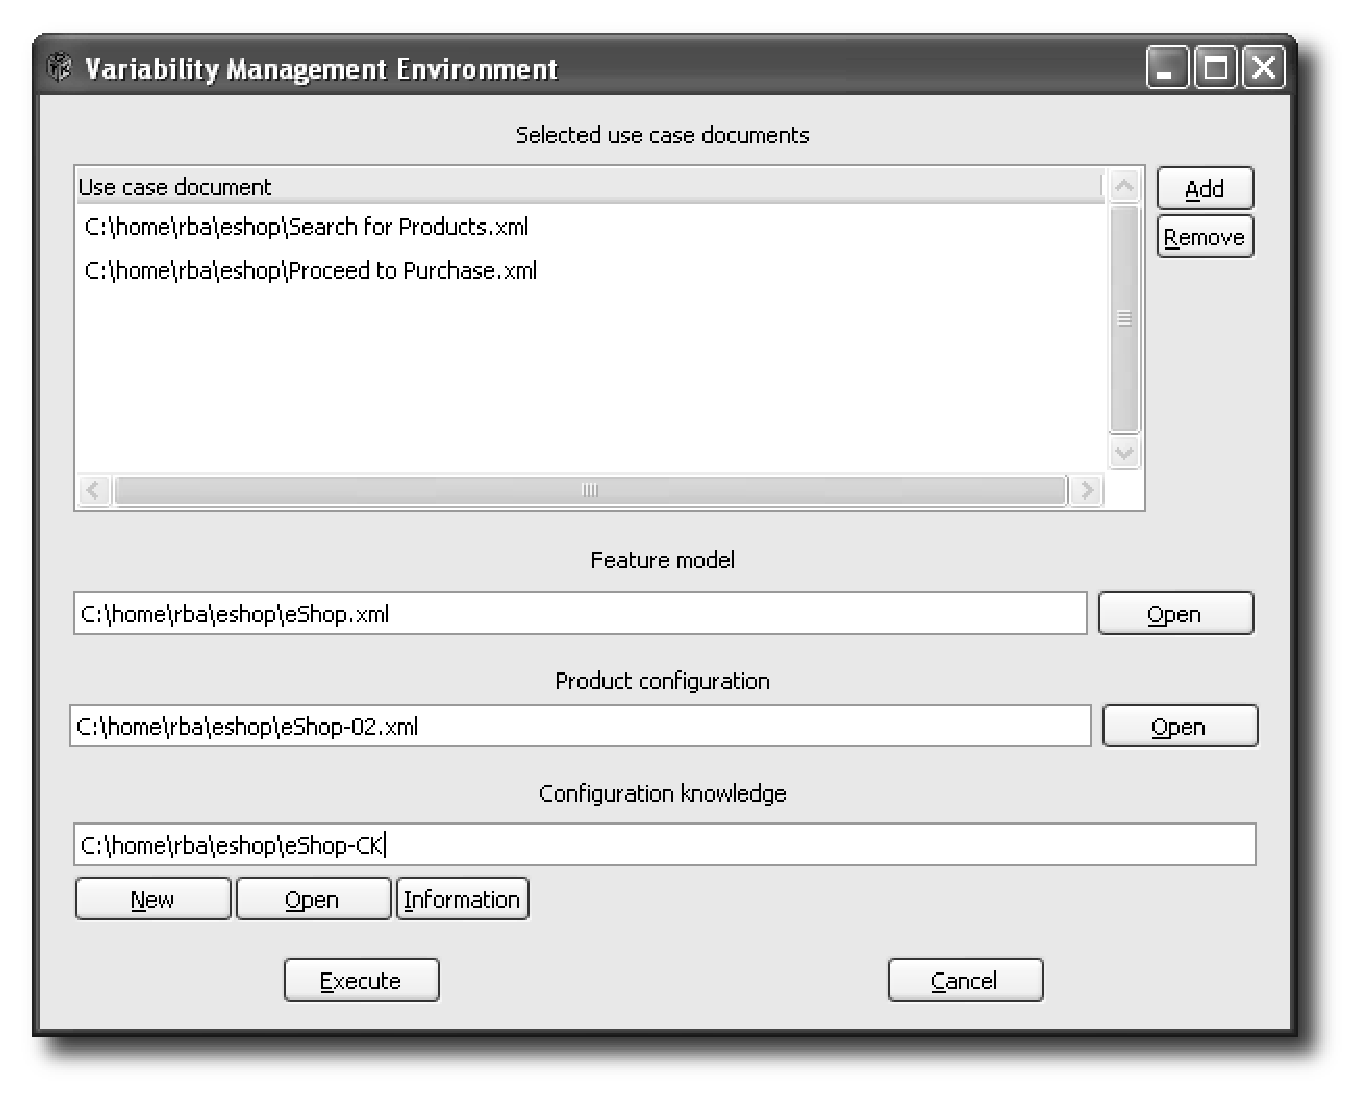
\includegraphics[scale=0.40]{img/msvcmTool.eps}
%    \caption{Weaving process' graphical environment.}
%   \label{fig:graphical-environment}
%   \end{center}
% \end{figure}
% 
% Similar to the weaving process, detailed in the next section, the tool support
% was also developed in Haskell, reusing common libraries for parsing XML documents
% (HXT) and graphical user interface (gtk2hasell). One overview of the major
% libraries and tools is shown in Figure~\ref{fig:haskell-libraries}.}
% 
% \begin{figure}[h]
%  \begin{center}
%   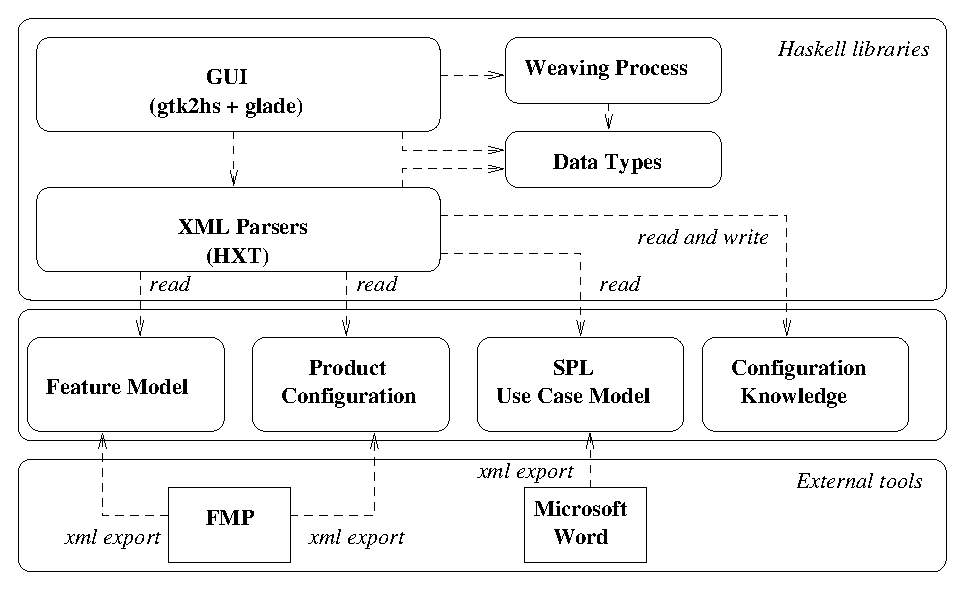
\includegraphics[scale=0.55]{img/architecture.eps}
%    \caption{Haskell libraries and external tools.}
%   \label{fig:haskell-libraries}
%   \end{center}
% \end{figure}


%There is no artifact similar to our configuration knowledge in
%PLUSS and PLUC approaches. As a consequence, introducing new variants of existing
%features in these techniques usually propagates changes throughout many
%scenarios.


%=================================================================
% Semantica do configuration knowledge
%=================================================================
% \begin{figure*}[hbt]
%  \begin{code}
%   (|->) :: a -> b -> (a,b) -- just a 'syntactic sugar' to build pairs
%   l |-> r = (l,r)
%
%   conf1 = Configuration (``eShop'' |-> selectScenarios[``SC01'', ``SC02''])
%   conf2 = Configuration ('Not' (``ShoppingCart'' 'And' ``Bonus'') |-> evaluateAdvice[``ADV01''])
%   conf3 = Configuration (``ShoppingCart'' 'And' ``Bonus'' |-> evaluateAdvice[``ADV02''])
%   conf4 = Configuration (``UpdateUserPreferences'' |-> evaluateAdvice[``ADV03''])
%   conf5 = Configuration (``ShipMethod'' |-> bindParameter(``ShipMethod'', `ShipMethod''))
%   ...
%
%   ck = [conf1, conf2, conf3, conf4, conf5]
%  \end{code}
% \caption{eShop configuration knowledge}
% \label{fig:ck-running-example}
% \end{figure*}
%
% We can reason about the effect of evaluating a configuration knowledge
% by means of trace models, defined to our context as:
%

%
% \begin{definition}
% A trace model is the set of valid sequences of events
% computed from the product scenarios. Events are labeled as the step ids of a
% scenario. The trace model for a scenario $s$ is given by:.
% \end{definition}
%
% \begin{code}
% traceModel s = traces (steps s)
% where
%   traces [] = [[]]
%   traces (x:xs) = [] : (stepId x) ^ (traces (xs))
%
% (^) :: (a -> [[a]]) -> [[a]]
% x ^ y = [ x:e | e <- y ]
% \end{code}
%
% For instance, Table~\ref{tab:ck-evaluation} presents the resulting trace models,
% after evaluating each configuration item of Figure~\ref{fig:ck-running-example}
% and considering the second product represented in
% Figure~\ref{fig:product-config-01-02}. Notice that the trace model of an empty
% product is the set with just one element: the empty sequence of events (not
% represented in Table~\ref{tab:ck-evaluation}).
%
% \begin{table}[hbt]
%   \begin{tabular}{{||m{0.3in} m{0.1in} p{0.05in} l||}}
%   	\hline
%  	Config 		  & Eval		 & & Trace Model  \\  \hline 	
%  	
%  	$conf1$		  & True	     & & \parbox[t]{2.4in} {
%  									 \raggedright
%  									 <>, <P1>, <P1,P2.sm>, <P1,P2.sm,P3>,
%  									 <S1>, <S1,S2>, <S1,S2,S3> \\
%  								    } 									
%     								\\ \hline
%     $conf2$		  & False	   & & \parbox[t]{2.4in} {
%  								   \raggedright
%  									 <>, <P1>, <P1,P2.sm>, <P1,P2.sm,P3>,
%  									 <S1>, <S1,S2>, <S1,S2,S3> \\
%  								  }
%  								 \\ \hline 										
% 	$conf3$		  & True	   & & \parbox[t]{2.4in} {
%  								   \raggedright
%  									 <>, <C1>, <C1,C2>, <C1,C2,P1>,
% 							         <C1,C2,P1,P2.sm>, <C1,C2,P1,P2.sm,P3>,
%  								     <S1>, <S1,S2>, <S1,S2,S3> \\
%  								   } 								
%  								 \\ \hline
% 	$conf4$		  & True	   & & \parbox[t]{2.4in} {
%  								   \raggedright
% 	                                <>, <C1>, <C1,C2>, <C1,C2,P1>,
% 							        <C1,C2,P1,P2.sm>, <C1,C2,P1,P2.sm,P3>,
% 							        <C1,C2,P1,P2.sm,P3,R1>,
%  								    <S1>, <S1,S2>, <S1,S2,S3>,
%  								    <S1,S2,S3,R1> \\
%  								   }   	
%  								 \\ \hline
% 	$conf5$		  & True	   & & \parbox[t]{2.4in} {
%  								   \raggedright
% 									<>, <C1>, <C1,C2>, <C1,C2,P1>,
% 							     <C1,C2,P1,P2.(Economical,Fast)>,
% 							     <C1,C2,P1,P2.(Economical,Fast),P3>,
% 							     <C1,C2,P1,P2.(Economical,Fast),P3,R1>
%  								 <S1>, <S1,S2>, <S1,S2,S3>,
%  								 <S1,S2,S3,R1> \\   	 							
%  								 }
%  								 \\ \hline	 						  	
%  				
%    \end{tabular}
% \caption{The effect of evaluating configuration items}
% \label{tab:ck-evaluation}
% \end{table}

%=================================================================
%=================================================================




% In what follows, we describe a high level view of the weaving process that
% combines the input languages in order to manage scenario variability.  Then, in
% Section~\ref{sub:modeling-framework} we formally present its semantics in terms
% of our modeling framework.

% \subsubsection{Weaving process}
%
% The weaving process represented in Figure~\ref{fig:weave-process} is responsible for performing the following activities:
%
% {\bf Validation activity:} This activity is responsible for checking if a product configuration is a valid instance of the feature model. If the product configuration is
% valid (it conforms to the relationship cardinalities and constraints of the feature model), the process might proceed.
%
% {\bf Product derivation activity:} This activity takes as input a (valid) product configuration and a configuration knowledge.
% Each feature expression of the configuration knowledge is checked against the product configuration. If the expression
% is satisfied, the related scenarios are assembled as the result of this activity. For the running example,
% Table~\ref{tab:assembled-scenarios} shows the assembled scenarios for the configurations depicted in Figure~\ref{fig:product-config-01-02}.
%
% \begin{table}[h]
% \begin{center}
% \caption{Assembled scenarios} \label{tab:assembled-scenarios}
% \begin{tabular}{ll}
%    \hline\noalign{\smallskip}
%   {\bf Configuration} & {\bf Assembled scenarios} \\
%    \noalign{\smallskip}
%    \hline
%    \noalign{\smallskip}
%     Configuration 1\hspace{15pt} & Proceed to Purchase \\
%                                                    & Search for Products \\
%                                                    & Buy a Product \\
%                              			  & \ldots \\
%    Configuration 2                        & Proceed to Purchase \\
%                              			  & Search for Products	 \\
% 			                           & Buy Products with Cart \\
%                                                    & Register User Preferences \\
%                              & \ldots       \\
%   \hline
% \end{tabular}
% \end{center}
% \end{table}
%
%  {\bf Scenario composition activity:} This activity is responsible for composing the scenarios assembled for a specific product configuration.
% Therefore, the resulting scenarios of the previous activity, which crosscut each other based on the \emph{From step} and \emph{To step clauses}, are woven. The
%  result is a use case model with complete paths (all \emph{From step} and \emph{To step} clauses are resolved).
%
% %  or a trace model (a set of all valid sequences of events extracted from the complete paths).
%
% The complete path is a high level representation, which uses the same constructions of the use case model (scenarios), and is illustrated here as a graph, where each node is labeled with a step id. For example, Figure~\ref{fig:complete-paths} depicts the complete paths for the first and second configurations of our running example. In the left side of the figure,  the composition of \emph{Buy a Product} with \emph{Proceed to Purchase} (branch labeled as B1, B2, P1, P2, P3) and \emph{Search for Product} (branch labeled as S1, S2, S3) scenarios are presented. Contrasting, on the right side of the figure, the results of this activity is presented for the second configuration. In this case, steps B1 and B2 have been replaced by steps V1 and V2 (because \emph{Shopping Cart} and \emph{Bonus} features are selected) and the step  R1 is introduced after steps P3 and S3 (because \emph{Update User Preferences} is selected in this configuration).
%
% %=====================
% % Trace model discussion
% %=====================
%
% %Instead, the trace model can be seen as a low level representation of the use case model. Such notation has a well defined semantic and might
% %be used for model checking and test case generation. Such applications of the trace model are beyond the scope of this paper. More information
% %can be found elsewhere\cite{csp-hoare,csp-roscoe,cfeitosa-sbmf-2006}. Here, the trace model is useful for implementing the last activity of our weave process, binding parameters, and
% %represents all possible sequences of events in a specific product configuration.
%
% %For instance, the trace model for the first configuration is the set of sequences:
%
% %\begin{small}
% %\begin{tabular}{rlc}
% %$Trace_{C1}$ = & \{<>, <idle>, <idle, 1S>, <idle, 1S, 2S>, \\
% %                    & <idle, 1S, 2S, 3S>,  <idle, 1S, 2S, 3S, end>, \\
% %                    & <idle, 1M>, <idle, 1M, 2M>, \ldots, \\
% %                    & <idle, 1M, 2M, 3M, 4M.ShipMethod, 5M, end> \}
% %\end{tabular}
% %\end{small}
%
% %========================
%
% % \begin{figure}[bth]
% % \begin{center}
% % \begin{tiny}
% % \begin{xy}
% % \xymatrix@R=10pt{
% % & *++[o][F-]{idle} \ar[r]\ar[d] & *++[o][F-]{B1} \ar[d]	& *++[o][F-]{idle} \ar[r]\ar[d] & *++[o][F-]{V1} \ar[d] 		\\
% % & *++[o][F-]{S1} \ar[d]  & *++[o][F-]{B2} \ar[d]           & *++[o][F-]{S1} \ar[d]  & *++[o][F-]{V2} \ar[d] 			\\
% % & *++[o][F-]{S2} \ar[d]  & *++[o][F-]{P1} \ar[d]           & *++[o][F-]{S2} \ar[d]  & *++[o][F-]{P1} \ar[d]			\\
% % & *++[o][F-]{S3} \ar[d]  & *++[o][F-]{P2} \ar[d]           & *++[o][F-]{S3} \ar[d]  & *++[o][F-]{P2} \ar[d] 			\\
% % & *++[o][F-]{end} & *++[o][F-]{P3} \ar[l]                     & *++[o][F-]{R1} \ar[d] & *++[o][F-]{P3} \ar[l]   			\\
% % &                         &                                                    &   *++[o][F-]{end}       &
% % }
% % \end{xy}
% % \end{tiny}
% % \caption{Complete paths represented  as a graph}
% % \label{fig:complete-paths}
% % \end{center}
% % \end{figure}
%
% {\bf Binding parameters activity:}  This activity weaves scenarios and product configurations in order to resolve all scenario parameters.
% For example, step P2 in Figure~\ref{fig:proceed-to-checkout} has a reference
%  to the \emph{ShipMethod} parameter, whose domain values are defined in the product configuration. For instance, in the first configuration depicted in Figure~\ref{fig:product-config-01-02}, the parameter \emph{ShipMethod} might assume the values \emph{Economical} or \emph{Fast}.
% In order to reduce the coupling between scenario specifications and feature model, a mapping is used for relating scenario parameters to features. In fact, this mapping is another input artifact of our modeling framework; but it was not represented in Figure because it was just introduced for avoiding explicit dependences between feature and use case models.
% Next, we introduce the modeling framework used to formally describe the weaving processes just presented.
% %===================
% % Trace model discussion
% %===================
%
% %For each trace that contains a parameterized event (or step), this activity creates a new trace for all of the possible parameter values. Consequently, resolving parameters for the trace $<idle,1M,2M,3M,4M.ShipMethod>$ results in the following sequences:
% %
% %\begin{center}
% %\begin{small}
% %\begin{tabular}{c}
% %<idle,1M,2M,3M,4M.Economical>, \\ <idle,1M,2M,3M,4M.Fast>, \\
% %\end{tabular}
% %\end{small}
% %\end{center}


